\documentclass[]{final_report}
\usepackage{graphicx}
\usepackage{hyperref}
\usepackage{listings}


%%%%%%%%%%%%%%%%%%%%%%
%%% Input project details
\def\studentname{Ciaran Palmer}
\def\projecttitle{SensorML on SenseTile}
\def\supervisorname{Your Supervisor Name}
\def\moderatorname{Your Moderator Name}


\begin{document}

\maketitle
\tableofcontents\pdfbookmark[0]{Table of Contents}{toc}\newpage

%%%%%%%%%%%%%%%%%%%%%%
%%% Your Abstract here

\begin{abstract}
SenseTileSensor Board

SensorML description.

WebServer to access sensor observations

SensorML Bon Mapping with a tool and method to develop sensorML descriptions

\end{abstract}




\newpage


%%%%%%%%%%%%%%%%%%%%%%
%%% Acknowledgments

\chapter*{Acknowledgments}

Vieri del Bianco , Dragan Stosic and Joseph R. Kiniry.

%%%%%%%%%%%%%%%%%%%%%%
%%% Introduction

\chapter{Introduction}

The aim of this thesis project was to model the SenseTile Sensor Board using Sensor Model Language (SensorML)\cite{SMLref} . A prototype of a Web Service for accessing SenseTile Sensor Board sensor observations was to be developed using this SensorML description of the SenseTile Sensor Board. An evaluation of the suitability of SensorML for use as part of the SenseTile System was also to be performed.

SenseTile is a sensor and processing package that can contain motion sensors, RFID sensors, temperature sensor, audio sensors, pressure sensors, light level sensors video sensors among others. It is used as a replacement for standard ceiling tiles to provide smart building services as part of a Web Sensor Network. The SenseTile System is made up of two units a Sensor Board and Processor Unit. The sensors are interfaced or hosted on the Sensor Board. The Processor Unit interfaces to the Sensor Board allowing data from the Sensor Board to be processed futher as required.

SensorML is one of a number of specifications provided by the Open Geospatial Consortium (OGC) as part of the Sensor Web Enablement(SWE) initiative[ref]. The members of the OGC have the goal of developing open standards to exploit Web connected sensors of all types. SensorML is used to describe sensor systems and the processing of sensor observations. It provides standard models and XML encodings to describe the process of sensor measurement. SensorML is described further in chapter x.

The SenseTile Web Service prototype allows access to the Sensor Board sensor observations and it's SensorML description. It runs on the SenseTile Processor Unit.  The Web Service is based on another OGC SWE  specification, the Sensor Observation Service (SOS)[ref]. This specification defines a standard Web interface for retrieving information about sensor systems and sensor observations. Sensor Board measurements that have been post processed and converted to real values or the raw Sensor Board data can be accessed using the Web Service. SOS Lite.

There are othe  SOS specification depend on another SWE specification, Observation and Measurements(O\&M)[ref]. This specification provides standard models and XML encoding for sensor observations.

A  SensorML to BON Mapping was also to be explored . BON\cite{BONref} is a notation and a method for Object Oriented systems analysis and design. Based on this mapping it was proposed to develop a tool/method to automatically generate SensorML descriptions. Generally SensorML is hand generated with all the shortcomings of such an approach. The proposed approach would allow sensor processing to defined formally in BON and then refined to JML/Java. 


\chapter{ Background Research}


\section{Sensor Web Enablement}
SensorML is developed as part of the Open Geospatial Consortium (OGC) Sensor Web Enablement (SWE) initiative (http://www.opengeospatial.org/projects/groups/sensorweb). This initiative is establishing interfaces and protocols to enable a standardized Sensor Web. It is hoped that this allows for easier integration and development of sensor applications across sensor networks. The OGC SWE provides a framework of open standards for use with Web-connected sensors and sensor systems. There are seven main specifications currently:

\begin{itemize}
\item  SensorModel Language(SensorML) - models and schema for sensor systems and processes surrounding measurements
\item  Sensor Observation Service (SOS) - standard web interface for accessing observations
\item  Observations \& Measurements (O\&M) - models and schema for packaging observation values
\item  Transducer Markup Language (TML) - models and schema for multiplexed data from sensor systems
\item  Sensor Planning Service (SPS) - standard web interface for tasking sensor systems and model and requesting acquisitions
\item   Sensor Alert Service (SAS) - standard web interface for publishing and subscribing to sensor alerts
\item   Web Notification Service (WNS) - standard web interface for asynchronous notification
\end{itemize}

SWE services based on the aboved specifications allow the discovery of sensors, access to the sensor data, as well as subscription to alerts, and tasking of sensors to con-trol observations. For a good overview of SWE and it's use in Sensor Web Network please see \cite{SWEArchref}

Rather than define any new sensor models or XML formats for SenseTile it preferable to use the existing solutions if good enough for the task at hand. The SWE framework seems to cover all that is needed for modeling sensors and observations. Support for easy exchange of sensor meta-data and sensor observations is the main rational of SWE and fits the needs of the SenseTile Sensor Network.  SensorML, SOS and O\&M specifications are the focus of this thesis and are described in more detail in the following sections.

\section{Sensor Modeling Language}
Sensor Modeling Language (SensorML) is primarily used to describe sensor systems and the processing of observations from sensor systems. The SensorML specification\cite{SMLref} provides a functional model of sensors and an XML encoding to describe sensors and their observations. Some of the main uses of SensorML described in the specification are:
\begin{itemize}
\item support sensor and sensor observation discovery
\item support processing of the sensor observations
\item support geolocation information about sensors
\item provide accuracy information of sensors measurements
\item Provide an explicit description of the process by which an observation was obtained
\item Provide an executable process chain for deriving new data products on demand
\end{itemize}

In SensorML sensors are modeled as processes that convert real phenomena to data. Processes take inputs, process them and result in one or several outputs. For example, a process can take a digital number generated by a thermistor and transform it to a celcius value. Processes can also be connected together in process chains to allow the sensor data to be processed by several processes sequentially. These processes and process chains are modeled in SensorML as shown in the  below SensorML Conceptual Model \ref{fig:SMLConceptualModel}.

\begin{figure}[h]
\framebox{\scalebox{0.65}{\includegraphics{SMLConceptualModel.png}}}
\caption{SensorML Conceptual Model}\label{fig:SMLConceptualModel}
\end{figure}

Processes in SensorML derive from AbstractProcess with it's inputs, output, parameters and metaDataGroup properties. The inputs and outputs represent data connections to other processes. Parameters represent inputs other than sensor measurements or outputs of other processes. They are used to configure the process or provide other inputs that are not sensor measurements. For example a parameter might be the latency time of a measurement needed for a calculation. Finally each process provides sensor metadata as modeled by the MetaDataGroup.

SensorML divides processes into two types, physical and non-physical. The non-physical process is one where  location, position etc. is not relevant to the process. Physical processes provide physical information, such as location, which can be used in processing if required. The ProcessModel is a non-physical process while the Component is a physical process and contains extra properties for defining the needed spatial or temporal information. Both process types contain the processMethod property which points to the methodology for transforming inputs to outputs.

There is a similar division of the process chains into the non-physical ProcessChain and physical System. Both process chains can contain a mixture of ProcessModel and Component process if desired. Process chains have inputs and outputs which define the beginning and end of the processing chain. They are points of connection to other processes and process chains if needed. The connection property contained in the ProcessChain and System is a list of Link type. The Link type contains source and destination propertes that reference inputs and outputs of the processes in the process chain thus connecting the processes. 

The SensorML specification currently contains the Sensor Web Enablement (SWE) Common specification. This specification defines basic types and data encodings used by the SWE specifications. It describes both primitive data types as well as aggregate types such as arrays and records. There are a large number of types defined in this specification, too many to show here. Below is a Conceptual Model of some of the simple data types.

\begin{figure}[h]
\framebox{\scalebox{0.65}{\includegraphics{SWESimpleConceptualModel.png}}}
\caption{SWE Common Simple Data Types.}\label{fig:SWESimpleConceptualModel}
\end{figure}

The data types in \ref{fig:SWESimpleConceptualModel} are scalar primitive values. They are the basis for the inputs, outputs and parameters in SensorML processes. Quantity models a floating point number. Count models a counting value or integer.  Boolean models a property that can be true or false. These types contain a number of properties that further define the type. The uom property provides a unit of measurement that indicate how the value should be interpreted.  A constraint property allows a value range or a enumerated list of values to be defined for the type. The quality property allows for a measure of its quality, for example the confidence level of a value being correct expressed as a percentage. Aggregation of these primitive data types is also provided by several types including DataRecord and DataArray.

It is stated in the SensorML specification that the SWE Common will be placed in it's own document in future releases. 

The XML encoding of the SensorML model is not described here. In section where a detailed description of a SensorML model of SenseTile is described.

\section{Sensor Observation Service}
SensorML is envisioned to be used in conjunction with a Sensor Observation Service as described in the SWE Architecture \cite{SWEArchref}. The SOS defines a web service interface for the discovery of sensors systems and the retrieval of observations from sensor systems. The SenseTile Web Service developed in this thesis is based on the concepts described in the Sensor Observation Service (SOS) specification.

The SOS specification uses four main entities to describe the SOS's operation. The entities are Data Consumers, Data Producers, OGC Catalogs and the SOS itself. Data Consumers are clients of the SOS that request sensor observations and sensor metadata. Data Providers are entities have to access to the sensor and have enough processing power to generate an XML encoding of the sensor's observations. These observations are sent over a network to the SOS. The OGC Catalog is used store metadata about the sensor systems and is used as part of the discovery process.

The diagram \ref{fig:SOSoperationContext} below shows the entities described in the SOS in an operation context
\begin{figure}[h]
\framebox{\scalebox{0.65}{\includegraphics{SOSoperationContext.png}}}
\caption{SOS Operational Context}\label{fig:SOSoperationContext}
\end{figure}

Collections of related sensor system observations are organized into Observation
Offerings. 

Observations are encoded as OGC O\&M Observations. Sensor systems metadata can be also be retrieved using the SOS interface and is generally defined in SensorML or TML.
para.  These operations are encoded in XML and used in http post and get operations. The XML message needs to be parsed to identify the operations, parameters and results. There seems to be work ongoing to change this to a more industry standard view of Web Services with the use of WSDL/SOAP. I could not find this as part of current OGC SWE framework.
para: Scalability would be achieved through aggregating a number of
sensor data producers on the sensor side and by aggregating a number of SOS instances
on the data center side for providing data to consumers. 
\subsection{SOS Data Consumer Operations}
There are there core operations that are provided by an SOS and used by SOS Clients to request sensor information:
 \begin{itemize}
\item GetObservation operation is used to obtain sensor observations and measurement data.
\item GetCapabilities operation is used to retrieve SOS service metadata.
\item DescribeSensor operation retrieves detailed information about the sensors.
\end{itemize}

\subsection{SOS Data Provider Operations}
Two other operations RegisterSensor and InsertObservation are of interest to this thesis. These are part of the SOS transactional interface. They are used with SOS data producers which are software entities connected to the sensor and have enough processing power to generate XML descriptions of the sensor data.

\subsection{SOS Catalogs}
The catalog aspect of SOS that used for discovery of the SOS instance is not covered in the Web Service Prototype described in this thesis. 
\subsection{Enhanced Operations}
Also six enhanced operations, GetResult,
GetFeatureOfInterest, GetFeatureOfInterestTime, DescribeFeatureOfInterest,
DescribeObservationType, and DescribeResultModel are not included in the SenseTileWeb Service.

\section{SenseTile}
A case study of the use of SensorML in sensor networks is based on the SenseTile System. SenseTile is a general purpose sensor system developed at UCD CASL (http://kind.ucd.ie/
products/opensource/SenseTile). The SenseTile System is used to investigate issues arising with large scale sensor networking. SenseTile is made up of a sensor platform, a datastore, and a compute farm.  The sensor platform is called the SenseTile Unit and is composed of one or more SenseTile Sensor Boards paired with a SenseTile Processor Unit. The Processor could be a PDA or small PC or any processing device that has a USB connection.  The Sensor Board has a USB connection and this is used for communication with the Processor Unit. There are over a dozen sensors on the SenseTile Sensor Board including a thermistor and light sensor. Sensors are mounted on the Sensor Board and more sensors can be added using the USB connection.

This SenseTile unit is where thesis will focus on the use of SensorML though SensorML can be used in other the parts of the SenseTile system. As the processor unit is  a relatively powerful computer, providing a Web Service on the SenseTile Unit is feasible. The part SensorML plays in this Web Service is explored in the context of the SenseTile system.


\section{UCD Sensor Board Driver}


\section{VAST SensorML Engine}
The VAST Team at the University of Alabama in Huntsville (UAH)  developed an open source JAVA based SensorML Processing Engine. This software parses SensorML and instantiates objects that implement SensorML processes and process  chains. The code is found at http://code.google.com/p/sensorml-data-processing/. It dependent on an implementation of the SWE Common data types described in the chapter on SensorML. This code can be found at call swe-common-data-framework http://code.google.com/p/swe-common-data-framework/. This software is referred to as the VastSMLEngine in rest of the thesis.


\section{BON}


\chapter{Design}
\section{SensorML Model of SenseTile}

A SensorML model of SenseTile is developed as part of this thesis. The model contains metadata about the SenseTile system and supports the needs of the SenseTile Web Service. Two main requirements of the SenseTile Web Service were to be supported by the SensorML model. Firstly the raw data from the senors is to be retrievable to allow external system process the data as desired. Secondly there is a requirement to do post processing on the Processor Unit of the sensor data to convert it to meaningful values. A block diagram of the Sensetile SensorML model is shown in figure \ref{fig:SenseTileSystem}.

\ref{fig:SensorML_SenseTile_System_comp}. Only the Thermistor Component and the Celcius Component are developed as part of this thesis. They are described in model detail in later sections.
\begin{figure}[h]
\framebox{\scalebox{0.65}{\includegraphics{SensorML_SenseTile_System_comp.png}}}
\caption{SenseTile System SensorML Block Diagram}\label{fig:SensorML_SenseTile_System_comp}
\end{figure}

Three SensorML Systems are used to model the SenseTile as shown in the block diagram. One SensorML System models the overall SenseTile which contains the Sensor Board and Conversion Systems. The below XML fragment shows how SensorML describes System containment using a component list and how the other SensorML Systems descriptions are referenced using xlink hrefs.

\lstset{language=XML,basicstyle=\scriptsize,frame=single}
\begin{lstlisting}
<sml:components>
        <sml:ComponentList>
               <sml:component name="sensorBoardSystem" 
                                          xlink:href="SensorBoardSystem.xml">
               </sml:component>
               <sml:component name="convertorSystem"  
                                          xlink:href="ConverterSystem.xml">
               </sml:component>
        </sml:ComponentList>			   
 </sml:components>
\end{lstlisting}

The physical phenomena measured by the sensors are the input to the  SenseTile System. These values will be read in from packets received from the Sensor Board. The Digital Number output is the raw sensor data which is a digital number without a physical meaning. The Converted Measurement output contains the values from post processing the sensor data which have some physical meaning such as temperature in Celcius.

The division of the systems is based on the concept that sensor observations are based on at least a sampling process and a conversion process{ref tutorial}. The Sensor Board System contains SensorML Components that model the sensors on the board that perform the sampling. The SensorML Components contained in the Conversion System model processes that produce meaningful physical measurement values such as temperature and lumens from the sampled data.

The SenseTile System connects up the inputs and outputs of the SensorBoard and Convertor Systems using SensorML connections. The below SensorML fragment shows how the temperature output from the SensorBoard System is connected to the input of the Conversion System is peformed in SensorML.
\newpage
\begin{lstlisting}
<sml:connection name="convertToTemperature">
    <sml:Link>
        <sml:source ref="sensorBoardSystem/outputs/temperatureDNOutput"/>
        <sml:destination ref="convertorSystem/inputs/celciusConvInput"/>
     </sml:Link>
 </sml:connection>
\end{lstlisting}



Naming rules for inputs and outputs - allow more generic handling of implementation classes.

System and components are in several files. Inline in one file if desired.Choice to seperate files.

\subsection{Thermistor Component}
The Thermistor on the SenseTile Sensor board is the Texas Instruments TMP175 Digital Temperature Sensor and is modeled with a SensorML Component. This is an indivisible process and can have a different location information than the Sensor Board if required. The SensorML Component allows the capabilities of the Thermsistor to be described. For example the TMP175 is  specified for operation over a temperature range of −40°C to +125°C. This is captured in the following SensorML:

\begin{lstlisting}
<swe:field name="TemperatureRange" 
           xlink:arcrole="urn:ogc:def:property:dynamicRange">
          <swe:QuantityRange definition="urn:ogc:def:property:temperature">
                   <swe:uom code="cel" /> 
                          <swe:value>-40 125/swe:value> 
           </swe:QuantityRange>
</swe:field>
\end{lstlisting}

The SensorML Thermistor temperature input is modeled using a Quantity value without any units as is a measured physical phenomena. Its output is a digital number from the sensor. The range is constrained to the allowed value range from the Thermistor. The following fragment shows how the input and outputs for the Thermistor look in SensorML:

\begin{lstlisting}
<sml:inputs>
    <sml:InputList>
         <sml:input name="thermistorInput">
             <swe:Quantity definition="urn:ogc:def:phenomenon:temperature">
         </sml:input>
    </sml:InputList>
</sml:inputs>

<sml:outputs>
    <sml:OutputList>
          <sml:output name="thermistorOutput">
               <swe:Count>
	        <swe:constraint>
                         <swe:AllowedValue id="outputRange">
                              <swe:interval>-880 2032</swe:interval>
                         </swe:AllowedValue>
                     </swe:constraint>
                </swe:Count>
           </sml:output>
     </sml:OutputList>
 </sml:outputs>
\end{lstlisting}


\subsection{Celcius Converter Component}

The SensoML Celcius Converter SensorML Component  models a process that performs a conversion of the Thermistors digital number output to a real quantity celcius value. It similar to the Thermistor SensorML description but its inputs and outputs are different. It process method performs a simple calcution to perform the celcius conversion.

A Sensor process method is also developed. The process method describes the coversion algorithm and points to an implementation class. Process Methods are not implemented by the Vast Lib so it not used in the running system. Instead the method tag provides a URN that is used to lookup the implementation class.

\section{BON to SensorML mapping}
Features to be elements or attributes.

Name rule suffix "Attrib" to make it an attribute.

List handling - convention for mapping.

SML prefix to handled key word clashes between sensorML and BON.


\section{SenseTile Web Service}
\subsection{Overview}

The SenseTile Web Service is based on the Sensor Observation Service (SOS) as described previously. The two main entities in the SOS Specification, the Sensor Data Provider and the SOS,  are used to structure the SenseTile Web Service. These entities are implemented as seperate software components that together provide the service. The Sensor Data Provider component will be referred to as the DataProvider in this design.

The two components are run as seperate processes on the SenseTile processor unit to allow a more flexible network architecture.  This network architecture is described in more detail in section \ref{subsec:SenseTile WebService Network Architecture}. The basic system structure is shown in figure \ref {fig:Deployment_sensetile} .

\begin{figure}[h]
\scalebox{0.65}{\includegraphics{Deployment_sensetile.png}}
\caption{SenseTile Web Service}\label{fig:Deployment_sensetile}
\end{figure}

The DataProvider parses a SensorML description of the SenseTile System, reads sensor data form the Sensor Board and provides the sensor data as O\&M Observations to the SOS. The SenseTile SOS will implement the SOS core operations to allow a client to get these observations. The following sections describe the design of the DataProvider and SOS components as well as the scenarios they support.

\subsection{Supported Scenarios}
\begin{table}[!th]
\begin{tabular}{|l|c|r|}
\hline
Scenarios\\
\hline
Generate Observations from Sensor Data \\
The DataProducer accesses data from the sensor board \\
\hline
Get Sensor Description from SOS\\
\hline
Get  Sensor Observation from SOS\\
\hline
\end{tabular}
\caption{Scenario Chart for SenseTile Web Service}
\label{ex:table}
\end{table}
\begin{figure}[h]
\framebox{\scalebox{0.65}{\includegraphics{InsertObs.png}}}
\caption{SensorML Conceptual Model}\label{fig:InsertObs}
\end{figure}

\begin{figure}[h]
\framebox{\scalebox{0.65}{\includegraphics{GetObs.png}}}
\caption{SensorML Conceptual Model}\label{fig:GetObs}
\end{figure}
\newpage
\subsection{SenseTile WebService Network Architecture}
\label{subsec:SenseTile WebService Network Architecture}
In the SenseTile Web Service the SOS acts as a gateway to the SenseTile Sensor Network. This prototype was designed with the network architecture as shown in fig \ref{fig:Deployment_network}. A client would access multiple SOS instances to get observations from the sensor network. An SOS could support several DataProducers and hence would not to be run on every SenseTile. 

\begin{figure}[h]
\scalebox{0.65}{\includegraphics{Deployment_sensetile_network.png}}
\caption{SenseTile Sensor Network Architecture}\label{fig:Deployment_network}
\end{figure}
The SOS Specification envisioned that the SOS would be run on a large external server as shown in fig \ref{fig:Deployment_ext_sos}. The DataProviders would update this external server with observations and clients would just access this large SOS.
\begin{figure}[h]
\scalebox{0.65}{\includegraphics{Deployment_sensetile_ext_sos.png}}
\caption{External SOS}\label{fig:Deployment_ext_sos}
\end{figure}
The SOS Specification describes the use of a Proxy SOS as shown in figure \ref{fig:Deployment_sos_aggr}. This architecture could be used with the SenseTile Sensor Network if accessing many SOSs is not feasible for the clients.
\begin{figure}[h]
\scalebox{0.65}{\includegraphics{Deployment_sensetile_sos_aggr.png}}
\caption{Proxy SOS}\label{fig:Deployment_sos_aggr}
\end{figure}

\newpage
\subsection{DataProducer}
The DataProducer's role, as described previously, is to read sensor data from the Sensor Board and generate O\&M observations. These observations are then sent to the SOS instance. The processing of the sensor data to generate the observations is described by the SensorML models. The DataProducer uses the OGC Vast Library to instantiate objects that implement the required data processing chains based on the SensorML models. The BON static diagram \ref{fig:bon_static_diagam_producer.png}
 shows the main clusters and classes of the DataProvider.

The SMLEngine cluster contains classes that provide access to
the Vast Lib that is providing the SensorML Engine.  The Vast Lib implemenation
of the SensorML Engine is hidden from the rest of the code thus.

The Sensors and Converters clusters contain classes that provide
implementation of process methods for SensorML components in the SensorBoard and
Converter SensorML Models respectively. These are referred to as sensor objects and
converter objects henceforth.

The DataProducer operates by repeating the below steps continously.
 \begin{enumerate}
\item Read Sensor Board Data
\item Process Sensor Data
\item Create O\&M Observations
\end{enumerate}
The steps above are detailed the in following sections with reference
to the BON static diagram \ref{fig:bon_static_diagam_producer.png}.

\subsubsection {1. Read Sensor Board Data}

The UCD SensorBoard Library is used by DataProducer to access
the data generated by the Sensor Board.
The library provides high level interface to the
the data from the sensor board. It reads data from the Sensor board and generates packets
containing the sensor data. These packets provide functionality
to access a particular sensors data such as the temperature
meaurement generated by the thermistor. 
This library is shown as the SensorBoard cluster in \ref{fig:bon_static_diagam_producer.png}
An instance of the class PacketInputStream to is used access the packets from the Sensor Board.

The DataProducer uses the Observer pattern to provide
packets to the SensorMLEngine for processing.
At start up the SenseTileSystem reads the list of sensor objects from the SMLEngine that
implement the Sensors interface. These objects provide an entry point
to the SensorML processing chain and can read data from the UCD LIB packets.
These sensor objects implement reading strategies for the type of data they read. 
For example the ThermistorSensor reads out the temperature value
but will average it before it sent to the SensorML Engine for processing.

\subsubsection {2. Process Sensor Data}
The PacketInputStream will request the SenseTileSystem to exexcute
the SensorML engine to process the sensor data. The SensoML Enigine
will execute the process chains described in the SenseTile SensorML model.
The sensor objects output will be passed to the coverter objects. The
outputs of both object types are then available to generate observations.

\subsubsection {3. Create O\&M Observations}

When the SensorML Engine is finished
and there are obsevations generated these
need to be sent to the SOS. An O\&M Onservation
xml string containing the data is sent to
the SOS instance. This is timestamped at
this stage.
 containing the output from
the SensorML processes and send the observations
to the SOS.
-register offerings with the SOS. In this design
each system is an offering.
Need to generate an observation model?


Questions.
If have light data but no temp. As temp is only
every 1000 packets?

How to know when to generate observation
for the two offerings?
DataProducer generates observations in Observation xml standard.

Interface to the SensorBoard Library.

Uses observer pattern to update sensors with packets from the board.

reads sensors from SensorBoard System xml

Sensors iimplement interface to facilitate this.

Vast lib connects all the processes

implementation of sensor and convertor is named using URN read from the sensorMl descption.


The DataProducer was developed as a SensorML based software. It would be parse the SenseTile SensorML model to instantiate the code to excute the processes described. This required two aspects to be developed, a framework to run the processes and classes that implemented the components.

\begin{figure}[h]
\scalebox{0.65}{\includegraphics{bon_static_diagam_producer.png}}
\caption{DataProducer Static Diagram}\label{fig:bon_static_diagam_producer.png}
\end{figure}

Interfaces to the Sensor Board


\newpage
\subsection {SOS}
 \begin{figure}[h!]
\scalebox{0.65}{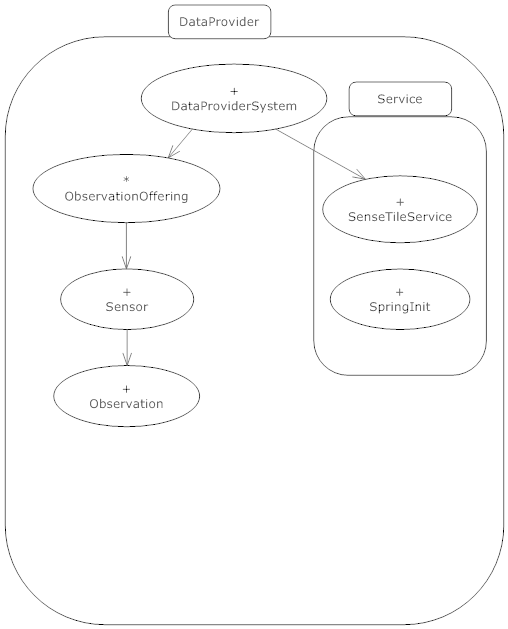
\includegraphics{bon_static_diagam_provider.png}}
\caption{SOS Static Diagram}\label{fig:bon_static_diagam_provider.png}
\end{figure}
Keeps track of sensorboards that register

provides an RMI interface to the DataProducer to update with observations. This has lower overhead
than a web service. Though it would not be hard to change to use a Web Service Interface.

GetObservaton - marshal Observation to xml string and send as response.

StreamObservation -  registered clients get new observation sent over UDP connection?

Provides a Web Service interface  based on Sensor Observation Service. Not fully as is a very complex interface.



\chapter{Implementation}

\section{DataProducer}

DataProducer VastLib UCD SenseTile Driver Lib

\section{SOS}
 is based on AXIS 2.0/Spring

JAXB for SensorML XML to java binding.

RMI used between DataProvider and SOS.

\section{SensorML Generation}

\chapter{Results}

running prototype tested with UCD SensorBoard Simulator code

Tested against real SenseTile and sensor data retrieved by a testclient.

Generation of SensorML description of a Senstile Sensor

\chapter{ Conclusions and Future Work}

what has been achieved

the weaknesses of your approach
SOS on the Processor Board. Is this right.

difficult schemas to program against.
JIBX did not generate a default binding.
Jaxb did with some help but did not generate the process type correctly.
Why?

Schemas cover all needs for sensor description and data.

A lot of schemas needed.

SWE not fully web services as W3C might define. Not SOAP. HTTP envelope
flexible.

Vast Lib use as a references only. Other ways such a XQUERY? XML techs?
As there are a large number of types etc. A quick way for a prototype.
Had to update library code to get it to work with the SenseTile Schemas. Schemas
passed the validation test tool from the site.

Portabiltiy, Vast Types POJOs.

Streaming the data.

\chapter{References}
\newpage
\begin{thebibliography}{99}
\bibitem{SMLref}Open Geospatial Consortium Inc., OpenGIS Sensor Model Language (SensorML) Implementation Specification, 2007
\bibitem{SOSref}Open Geospatial Consortium Inc.,  Sensor Observation Service, 2007
\bibitem{OMref}Open Geospatial Consortium Inc., Observations and Measurements – Part 1 - Observation schema, 2007
\bibitem{SWEArchref}Open Geospatial Consortium Inc., OGC Sensor Web Enablement Architecture, 2008
\bibitem{SMLTutorialref}Open Geospatial Consortium Inc., Using SensorML to describe a
Complete Weather Station , 2006
\bibitem{ProcessTutorialref}Open Geospatial Consortium Inc.,

\bibitem{BONref}Kim Waldén and Jean-Marc Nerson , "Seamless Object-Oriented Software Architecture", 1995
\end{thebibliography}
\label{endpage}


\chapter{Appendices}

\lstinputlisting{Thermistor.xml}





\end{document}

\end{article}
